\hypertarget{group__x_event_group_set_bits_from_i_s_r}{}\section{x\+Event\+Group\+Set\+Bits\+From\+I\+SR}
\label{group__x_event_group_set_bits_from_i_s_r}\index{x\+Event\+Group\+Set\+Bits\+From\+I\+SR@{x\+Event\+Group\+Set\+Bits\+From\+I\+SR}}
Collaboration diagram for x\+Event\+Group\+Set\+Bits\+From\+I\+SR\+:\nopagebreak
\begin{figure}[H]
\begin{center}
\leavevmode
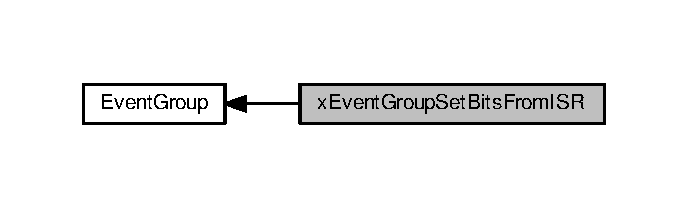
\includegraphics[width=330pt]{group__x_event_group_set_bits_from_i_s_r}
\end{center}
\end{figure}
\hyperlink{event__groups_8h}{event\+\_\+groups.\+h} 
\begin{DoxyPre}
   BaseType\_t \hyperlink{event__groups_8h_a62b68278abac6358369ae8e390988a02}{xEventGroupSetBitsFromISR( EventGroupHandle\_t xEventGroup, const EventBits\_t uxBitsToSet, BaseType\_t *pxHigherPriorityTaskWoken )};
\end{DoxyPre}


A version of \hyperlink{event__groups_8h_a02d7b3bb55f7e11d9c47116266c5fb2e}{x\+Event\+Group\+Set\+Bits()} that can be called from an interrupt.

Setting bits in an event group is not a deterministic operation because there are an unknown number of tasks that may be waiting for the bit or bits being set. Free\+R\+T\+OS does not allow nondeterministic operations to be performed in interrupts or from critical sections. Therefore \hyperlink{event__groups_8h_a62b68278abac6358369ae8e390988a02}{x\+Event\+Group\+Set\+Bits\+From\+I\+S\+R()} sends a message to the timer task to have the set operation performed in the context of the timer task -\/ where a scheduler lock is used in place of a critical section.


\begin{DoxyParams}{Parameters}
{\em x\+Event\+Group} & The event group in which the bits are to be set.\\
\hline
{\em ux\+Bits\+To\+Set} & A bitwise value that indicates the bit or bits to set. For example, to set bit 3 only, set ux\+Bits\+To\+Set to 0x08. To set bit 3 and bit 0 set ux\+Bits\+To\+Set to 0x09.\\
\hline
{\em px\+Higher\+Priority\+Task\+Woken} & As mentioned above, calling this function will result in a message being sent to the timer daemon task. If the priority of the timer daemon task is higher than the priority of the currently running task (the task the interrupt interrupted) then $\ast$px\+Higher\+Priority\+Task\+Woken will be set to pd\+T\+R\+UE by \hyperlink{event__groups_8h_a62b68278abac6358369ae8e390988a02}{x\+Event\+Group\+Set\+Bits\+From\+I\+S\+R()}, indicating that a context switch should be requested before the interrupt exits. For that reason $\ast$px\+Higher\+Priority\+Task\+Woken must be initialised to pd\+F\+A\+L\+SE. See the example code below.\\
\hline
\end{DoxyParams}
\begin{DoxyReturn}{Returns}
If the request to execute the function was posted successfully then pd\+P\+A\+SS is returned, otherwise pd\+F\+A\+L\+SE is returned. pd\+F\+A\+L\+SE will be returned if the timer service queue was full.
\end{DoxyReturn}
Example usage\+: 
\begin{DoxyPre}
  #define BIT\_0 ( 1 << 0 )
  #define BIT\_4 ( 1 << 4 )\end{DoxyPre}



\begin{DoxyPre}  // An event group which it is assumed has already been created by a call to
  // xEventGroupCreate().
  EventGroupHandle\_t xEventGroup;\end{DoxyPre}



\begin{DoxyPre}  void anInterruptHandler( void )
  \{
  BaseType\_t xHigherPriorityTaskWoken, xResult;\end{DoxyPre}



\begin{DoxyPre}    // xHigherPriorityTaskWoken must be initialised to pdFALSE.
    xHigherPriorityTaskWoken = pdFALSE;\end{DoxyPre}



\begin{DoxyPre}    // Set bit 0 and bit 4 in xEventGroup.
    xResult = xEventGroupSetBitsFromISR(
                        xEventGroup,    // The event group being updated.
                        BIT\_0 | BIT\_4   // The bits being set.
                        \&xHigherPriorityTaskWoken );\end{DoxyPre}



\begin{DoxyPre}    // Was the message posted successfully?
    if( xResult == pdPASS )
    \{
        // If xHigherPriorityTaskWoken is now set to pdTRUE then a context
        // switch should be requested.  The macro used is port specific and
        // will be either \hyperlink{portmacro_8h_aac6850c66595efdc02a8bbb95fb4648e}{portYIELD\_FROM\_ISR()} or \hyperlink{portmacro_8h_a63b994040c62c9685490a71c87a13d8a}{portEND\_SWITCHING\_ISR()} -
        // refer to the documentation page for the port being used.
        \hyperlink{portmacro_8h_aac6850c66595efdc02a8bbb95fb4648e}{portYIELD\_FROM\_ISR( xHigherPriorityTaskWoken )};
    \}
 \}
  \end{DoxyPre}
 